\section{Background and Main Ideas}

\jn{Add a pre-text to describe the structure of this section}

\subsection{Data Cleaning is Often Expensive}
A number of surveys of analysts report that data cleaning is one of the most time consuming steps \cite{kandel2012enterprise, nytimes}.
A number of data cleaning frameworks have been recently proposed to address the problem of corrupted data at scale\cite{khayyat2015bigdansing, chu2015katara, sampleclean}.
As errors can be domain- or dataset-specific, data cleaning is an inherently human-driven process and can require a significant amount of developer effort in writing software or rules to fix the corruption.
Automated fixes may not be reliable and can require human confirmation \cite{DBLP:journals/pvldb/YakoutENOI11}.
One way to scale up human computation is crowdsourcing which has shown recent success in entity resolution and value filling \cite{gokhale2014corleone, park2014crowdfill, sampleclean,chu2015katara}.
However, crowdsourcing comes with the costs of significant additional latency (orders of magnitude slower than data processing) and the overhead of managing human workers.

\subsection{Traditional Approximate Query Processing}

\jn{Add a section here to show the background of approximate query processing, and say it has a quite different idea from ours: it is for query time but not for query quality. }

\subsection{Exploiting Application Structure}

\jn{It's a little too early to present the content of this section before showing the big idea. I would suggest to put it either to the end of Sec 2 or the end of Sec 3. }

SampleClean applies sample to clean $k\ll N$ rows in a database to address the time-scale mismatch between the analytics application (e.g., SQL query, Machine Learning, Materialized View) and data cleaning.
An important aspect of this project is how the structure and semantics of that application can be used to prioritize and budget data cleaning.
A database only needs to be sufficiently clean for the requirements of the subsequent analytics--and the key insight from AQP being that aggregates are tolerant to approximation.

In the initial SampleClean work, we restricted the allowed aggregate queries to \sumfunc, \countfunc, and \avgfunc with predicates and group by clauses.
In the two subsequent projects, View Cleaning and ActiveClean, we expanded the scope and the semantics of the application. 
The View Cleaning problem explores data cleaning and general aggregates on derived relations with known view definitions.
We can exploit view definition to query just as much of the base data as needed to accurately answer the aggregate query for a fixed budget.
In fact, we showed that any aggregate (beyond \sumfunc, \countfunc, and \avgfunc) that could be estimated with SAQP\cite{agarwalknowing}, could be answered estimated with the View Cleaning framework.
ActiveClean generalizes the initial work on \sumfunc, \countfunc, and \avgfunc to higher-dimensional aggregates.
We defined a class of analytics called Convex Data Analytics, and show how the convex structure of the analytics can be used to guide and prioritize data cleaning.

\subsection{Approximate Query Processing on Dirty Data}


\subsubsection{Two Sources of Errors: Sampling Error and Data Error}

\jn{You may need to change the first paragraph as we add the Sec 2.2.}

To understand how we can integrate data cleaning and sampling, let us first understand how traditional AQP is affected by dirty data.
Sampling-based approximate query processing (SAQP) is a powerful technique that allows for fast approximate results on large datasets. 
It has been well studied in the database community since the 1990s~\cite{DBLP:conf/sigmod/HellersteinHW97,DBLP:conf/sigmod/AcharyaGPR99}\jn{Cite Olken et al. VLDB 1986}, and methods such as BlinkDB~\cite{DBLP:conf/eurosys/AgarwalMPMMS13} have drawn renewed attention in recent big data research. 
An important aspect of SAQP is confidence intervals, as many types of aggregates can be bounded with techniques such as concentration inequalities (e.g., Hoeffding bounds), large-deviation inequalities (e.g., Central Limit Theorem), or empirically (e.g., bootstrap).
However, these bounds assume that the only source of error is uncertainty introduced by sampling, however, the data itself may contain errors which could also affect query results. 


Suppose, there is a relation $R$ and a uniform sample $S$.
SAQP applies a query $q$ to $S$ (possibly with some scaling $c$) to return an estimate: \jn{``e" looks like an abbreviation for ``error". I would suggest to use a different one, e.g., ``est".}
\[
q(R) \approx e = c \cdot q(S)
\]
If $R$ is dirty, then there is a true relation $R_{clean}$.
\[
q(R_{clean}) \ne q(R) \approx e = c \cdot q(S)
\]
The error in $e$ has two components error due to sampling $\epsilon_s$ and error due to the difference with the cleaned relation $\epsilon_c = q(R_{clean}) - q(R)$:
\[
\mid q(R_{clean}) - e \mid \le \epsilon_s + \epsilon_c
\]

While they are both forms of query result error $\epsilon_s$ and $\epsilon_c$ are very different quantities.
$\epsilon_s$ is a random variable due to the sampling, and different samples would result in different realizations of $\epsilon_s$.
As a random variable introduced by sampling, $\epsilon_s$ can be bounded by a variety of techniques as a function of the sample size.
On the other hand, $\epsilon_c$ is deterministic, and by definition is a unknown quantity until all the data is cleaned.
Thus, the bounds returned by a typical AQP framework on dirty data would neglect $\epsilon_c$.

It is possible that $R_{clean} \ne R$ but $\epsilon_c=0$.
Consider a \sumfunc query on the relation $R(a)$, where $a$ is a numerical attribute.
If half of the rows in $R$ is corrupted with $+1$ and the other half are corrupted with $-1$, then $q(R_{clean}) = q(R)$.
In the data cleaning setting, we are interested in \emph{systematic errors} where $\epsilon_c > 0$ \cite{taylor1982introduction}. 
In other words, the corruption that is correlated with the data, e.g., where every record is corrupted with a $+1$.

\subsubsection{Key Idea I: Direct Estimate vs. Correction}
The key quantity of interest in this work is $\epsilon_c$, and essentially, to be able to bound
a query result on dirty data we need to either ensure $\epsilon_c$ is 0 or bound $\epsilon_c$.
We need to be able to ensure this for all budgets $k$ \jn{It's impossible for small $k$. Remove it or avoid saying ``all" }.
In particular, there are two ways in which this can be done: direct estimates and corrections.

\vspace{0.5em}
\noindent\textbf{Direct Estimate (Figure \ref{fig:est}A): } This technique is a direct extension of SAQP to handle data cleaning. Suppose, we want to estimate the query $Q$ on a dirty relation $R$. A set of $k$ rows is sampled uniformly at random from the dirty relation $R$ resulting in a sample $S$. Data cleaning is applied to the sample $S$ resulting in $S_{clean}$.
Data cleaning and sampling may change the statistical and scaling properties of the query $Q$, so $Q$ may have to be re-written to a query $\widehat{Q}$. $\widehat{Q}$ is applied to the sample $S_{clean}$ and the result is returned. 
There are a couple of important points to note about this techniques.
First, as in SAQP, the direct estimate only processes a sample of data.
Next, since it processes a cleaned sample of data, at no point is there a dependence on the dirty data.
As we will show later in the paper, the direct estimate returns a result whose accuracy is independent of the magnitude or rate of data error. 
From a theoretical perspective, for some types of data cleaning, this technique ensures that $\epsilon_c = 0$ within the sample.

\vspace{0.5em}
\noindent\textbf{Correction (Figure \ref{fig:est}B): } The direct estimate suffers a subtle drawback. Suppose, there are relatively few errors in the data. The errors introduced by sampling may dominate any error reductions due to data cleaning. Instead of the direct estimate which ensures $\epsilon_c = 0$, we can try to estimate $\epsilon_c$. A set of $k$ rows is sampled uniformly at random from the dirty relation $R$ resulting in a sample $S$. Data cleaning is applied to the sample $S$ resulting in $S_{clean}$. 
If we look at the difference in applying $\widehat{Q}$ to S and to $S_{clean}$, we can estimate the error $\epsilon_c$. 
This allows us to issue a correction to the query result on the full data.
In contrast to the direct estimate, this technique requires processing the entire dirty data (but only cleaning a sample).
However, as we will later show, if errors are rare this technique gives significantly improved accuracy over the direct estimates.

\begin{SCfigure}\centering
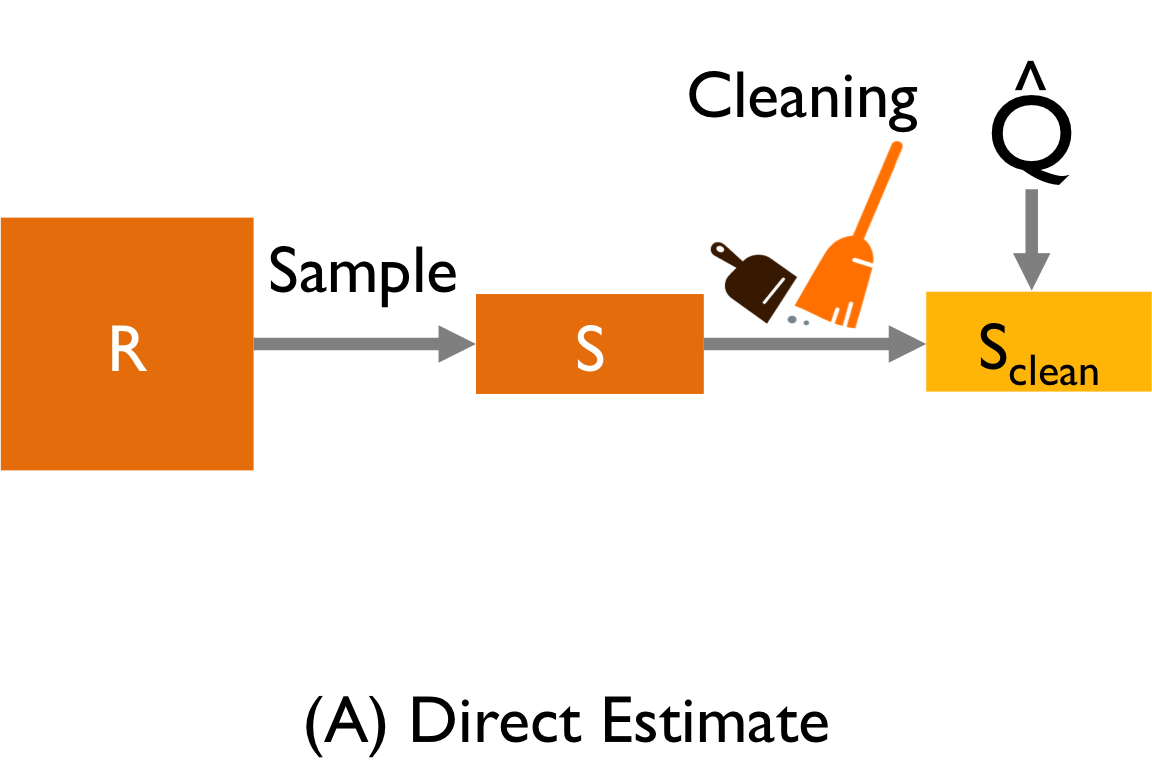
\includegraphics[width=.3\columnwidth]{figs/est1b.png}
\hspace{2em}
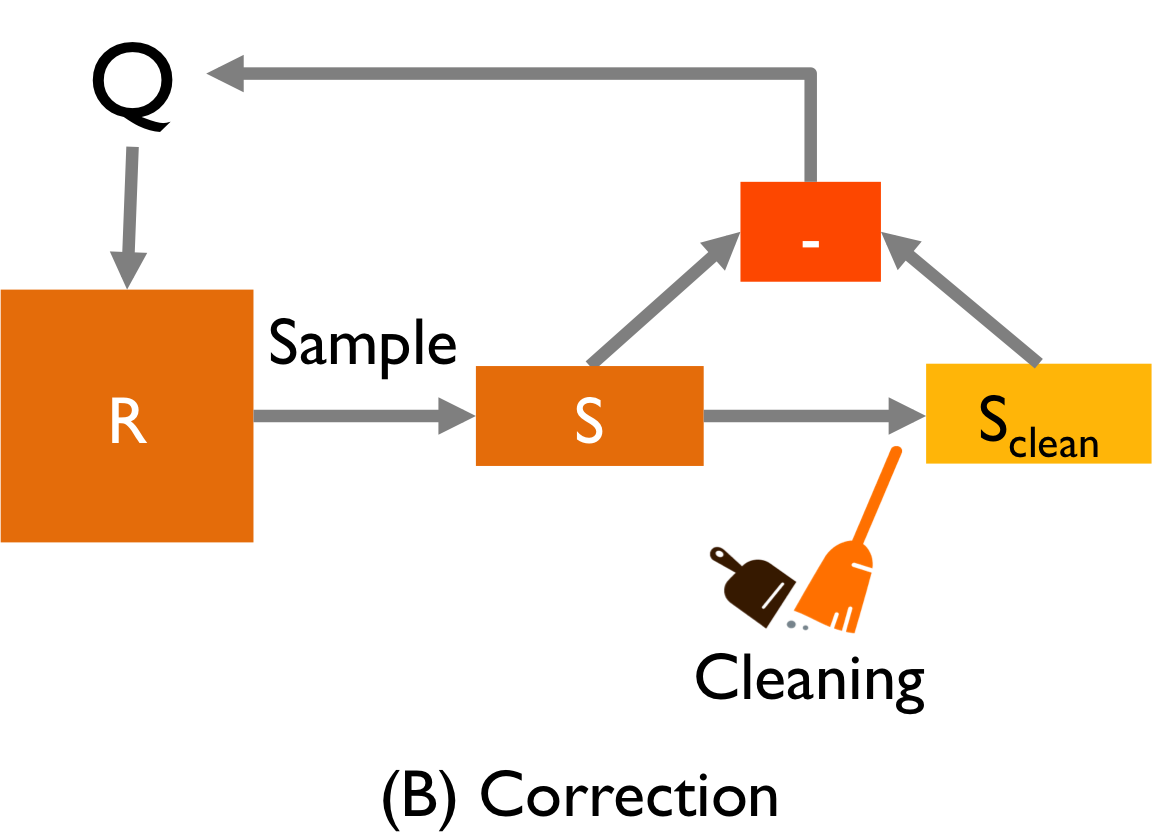
\includegraphics[width=.3\columnwidth]{figs/est1c.png}
\caption{Estimating query results with data cleaning on random samples. There are two ways to estimate a query result: (a) direct estimation applies the query to a sample (possibly with some scaling), and (b) correction corrects a query result on the entire dirty data.\label{fig:est}}
\end{SCfigure}

\subsubsection{Key Idea II: Sampling to Improve Accuracy}
The main argument for SampleClean is that when data errors significantly affect query results, a small sample of clean data can improve accuracy.
This is a counter-intuitive point since traditionally AQP sacrifices accuracy due to sampling; however, when sampling is combined with data cleaning it is possible that a query on a cleaned sample is more accurate than a query on the entire dirty data.
To better understand this tradeoff, we illustrate one of the experiments from SampleClean \cite{wang1999sample}.
In Figure \ref{fig:est2}, we plot error as a function of the cleaned sample size on a corrupted TPCH dataset.
\jn{It seems that you forgot to say that SampleClean achieved better accuracy than ALLDirty in the experimental description, which is the main point of this section.}
When errors are relatively rare (5\% corruption rate), the correction is more accurate. 
When errors are more significant (50\% corruption rate), the direct estimate is more accurate.
Note that the direct estimate returns results of the same accuracy regardless of the corruption rate. 



\begin{SCfigure}
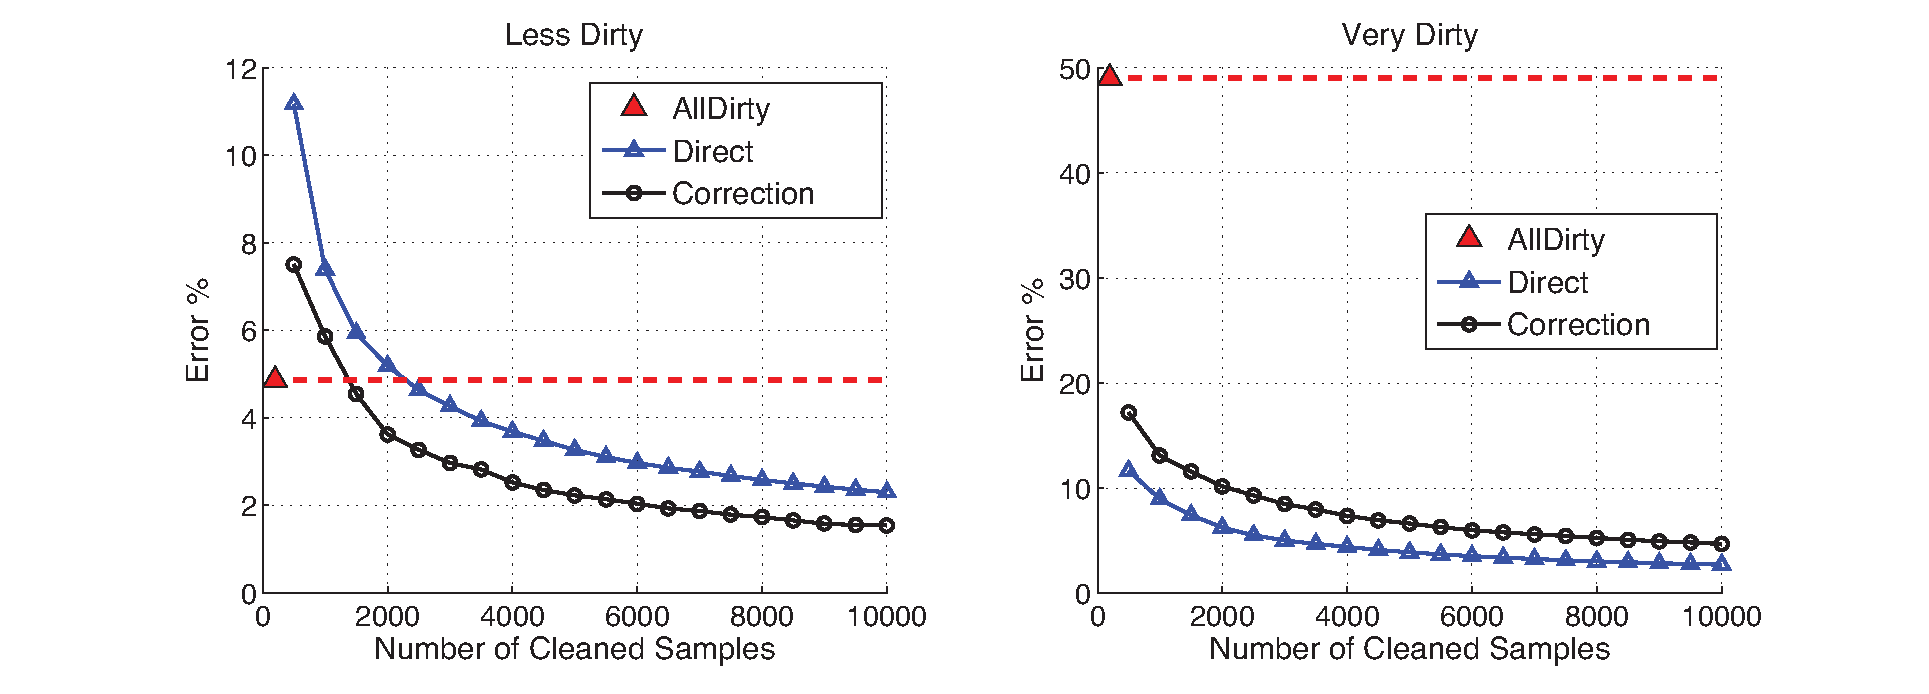
\includegraphics[width=.6\columnwidth]{figs/allerror-samplesize.eps}
\caption{Comparison of the convergence of the methods on two TPC-H datasets of 6M tuples with simulated errors 50\% error and 5\% error. On the dataset with larger errors, we find that the direct estimate gives a narrower confidence interval, and on the other the correction is more accurate. \jn{Enlarge the font size in the figure}  \label{fig:est2}}
\end{SCfigure}



